\documentclass[../main.tex]{subfiles}
\graphicspath{{\subfix{../images/}}}
\begin{document}

% \subsubsection{Camera Calibration} \label{sec:camera_intriniscs_results}

Camera calibration was performed using a newly fabricated checkerboard target, shown in Figures~\ref{fig:checkerboard_old} and~\ref{fig:checkerboard_new}.  
The target consists of a 6$\times$9 grid of 100~mm squares, providing 40 corner features for registration.  
Thirty HDR images were captured with the checkerboard placed at positions spanning the horizontal field of view and distances between five and 40~m.
These images were then processed with MATLAB Camera Calibration app \cite{matlab_calibration}, which was successful in detecting the checkerboard in 23 separate frames.  
This initial process provided a set of camera intrinsic values with a mean pixel error of 0.63~pixels (Figure~\ref{fig:HDR_calib_error}).

% \begin{figure}[htbp]
%     \centering
%     \includegraphics[width=0.9\linewidth]{Images/checkerboard_old.jpg}
%     \caption{Older paper-based checkerboards maintained dimensional accuracy but degraded over time.}
%     \label{fig:checkerboard_old}
% \end{figure}

% \begin{figure}[htbp]
%     \centering
%     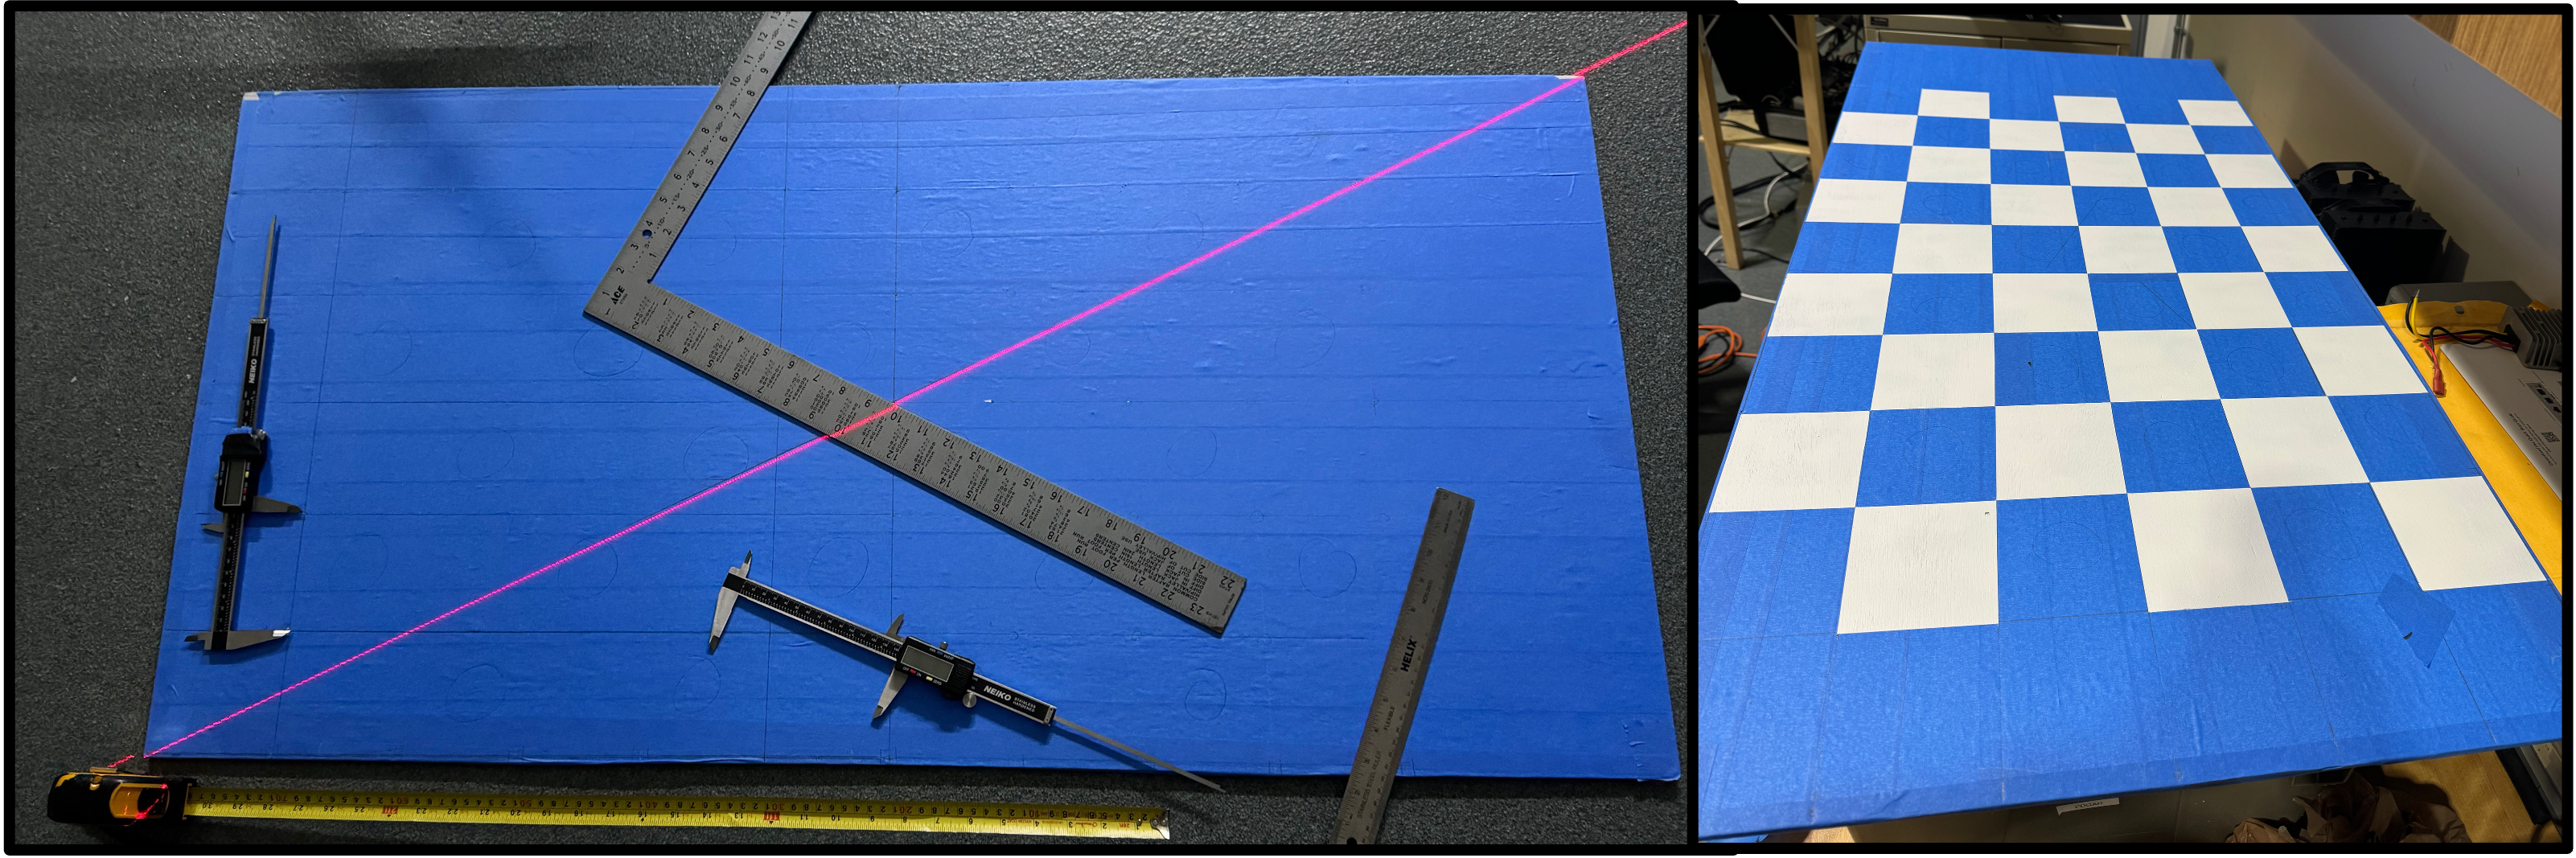
\includegraphics[width=0.9\linewidth]{Images/Checkerboard_new.png}
%     \caption{New precision-painted checkerboard target used for intrinsic calibration.}
%     \label{fig:checkerboard_new}
% \end{figure}

% \begin{figure}[htbp]
%     \centering
%     \includegraphics[width=0.9\linewidth]{Images/HDR_calib_error.png}
%     \caption{Initial HDR camera calibration yielded a mean re-projection error of 0.63~pixels across the dataset.\textcolor{red}{reproduce graphic with larger text and landscape orientation. no need for square aspect ratio.}}
%     \label{fig:HDR_calib_error}
% \end{figure}

% The resulting transformation achieved sub-degree rotational and centimeter-level translational accuracy, sufficient for reliable fusion and object detection.

\end{document}